Per attuare questo confronto tra mezzi di trasporto si è scelto di appoggiarsi a servizi di navigazione in grado di fornire stime di percorrenza (Estimated time of arrival, ETA) in tempo reale e usarle come valori effettivi. Le gare per confrontare tali mezzi sono state tradotte in richieste di stime di percorrenza per un tragitto comune a tutti, effettuate più volte al giorno e per diversi percorsi. In questo modo si è riusciti nell'intento iniziale di effettuare uno studio su degli stessi percorsi iniziati nello stesso momento ma con mezzi di trasporto diversi.

\section{Mezzi di trasporto e relativi servizi}

Sono stati presi in considerazione i principali mezzi di trasporto alternativi all'automobile di proprietà con cui è possibile spostarsi all'interno del Comune di Milano: servizio di car sharing, mezzi pubblici e passanti ferroviari, bicicletta di proprietà e infine il percorso a piedi. Quest'ultimo, anche se non diretto competitor, è stato scelto per essere usato come riferimento.

\subsection{Ricerca delle A.P.I}

Il primo passo verso la scrittura di un software per effettuare le varie richieste di percorso è stata quella di cercare delle API disponibili per ogni mezzo di trasporto in grado di fornire stime dinamiche sui tempi di percorrenza basate su dati in tempo reale.

\subsubsection{Google (auto, bici e a piedi)}

Inevitabilmente Google è stata la prima opzione che si è cercata. Google infatti, grazie a Maps e grazie all'acquisizione di Waze\cite{googleblog}, è una dei leader nel settore delle informazioni di navigazione e che vende la loro conoscenza tramite API. Tra le varie API offerte è presente quella che fa il caso di questo studio, la Directions API, che è in grado di fornire stime di percorrenza molto precise per l'auto, per il percorso a piedi e per la bicicletta (quando disponibile)\cite{googleapi}. Purtroppo però, il costo per l'utilizzo di queste API è di 10\$ per 1000 richieste al mese, l'equivalente di circa 1 richiesta all'ora, che risulta troppo poco per l'obbiettivo dello studio di catturare la variazione delle performance dei mezzi di ora in ora\cite{googleapiprice}.

\subsubsection{Waze (auto)}

Nonostante sia stata acquisita da Google, Waze è rimasta indipendente a livello di API. Quello che offre Waze però non è esattamente un endpoint a cui fare richiesta per un determinato viaggio, ma semplicemente degli URL da inserire nel proprio sito web o nella propria app Android/iOs per aprire il client Waze da browser/app coi dati della richiesta parametrizzati nell'URL\cite{wazeapi}.

\subsubsection{Moovit (mezzi pubblici)}

Anche Moovit non offre API per interrogare direttamente i loro servizi e ricevere delle stime, ma solamente l'opzione di incorporare un widget all'iterno della propria pagina web o applicazione che rimanda direttamente ai loro servizi\cite{moovitapi}.

\subsubsection{Here (auto, scooter e mezzi pubblici)}

Il servizio Here offre una REST API per le informazioni riguardo il routing e la stima del tempo di percorrenza. Queste stime però risultano accurate (basate su dati in tempo reale) solo per determinate città, comunicate sul loro sito, e tra queste non è inclusa Milano. Per le città non in lista, la stima è fatta sulla base dei dati tabellari degli orari dei passaggi dei mezzi\cite{hereapi}.

\subsubsection{Car2Go, Enjoy (car sharing)}

Non sono stati trovati servizi relativi a stime di tempi di percorrenza utilizzando un mezzo dei servizi car sharing. I servizi di car sharing Car2Go ed Enjoy non offrono API per tale calcolo ma dispongono di una mappa costantemente aggiornata sul loro sito web con l'elenco delle auto libere, ognuna con allegato dati riguardo il tipo di veicolo (tra auto e moto) e il carburante rimasto. Un programma in grado di acquisire le informazioni delle auto libere è stato gentilmente offerto da Federico Losacco, che lo ha scritto e utilizzato per uno studio sul comportamento del traffico basato sui viaggi compiuti dagli utenti del servizio\cite{losaccofederico}.

\subsubsection{OpenStreetMap e dintorni (auto, bici e a piedi)}

Il progetto collaborativo di OpenStreetMap offre, tra le altre cose, il calcolo di un tragitto usando come backend servizi offerti da terze parti, tra cui Open Source Routing Machine (OSRM). Purtroppo però, tali servizi non usano dati in tempo reale per la stima del tempo di percorrenza\cite{osm}.

\subsection{Scelta delle API}

Di seguito sono elencate le scelte fatte per i servizi e i loro rispettivi ruoli di copertura dei mezzi di trasporto:

\begin{itemize}
	\item HERE REST API\cite{herewegoapi}
	\begin{itemize}
		\item mezzi pubblici ATM e passanti ferroviari;
	\end{itemize}

	\item OpenStreetMap con OSRM\cite{openstreetmap}
	\begin{itemize}
		\item bicicletta di proprietà e a piedi;
	\end{itemize}

	\item Enjoy Map scraper di Federico Losacco\cite{enjoycarsharing}\cite{losaccofederico}
	\begin{itemize}
		\item posizioni delle auto libere Enjoy (car sharing);
	\end{itemize}
\end{itemize}

Nonostante OSRM non offra soluzioni in tempo reale ma statiche, è stato scelto ugualmente per via della scarsa influenza del traffico sui tempi di pecorrenza in bicicletta e a piedi, che dipendono per la maggior parte dall'itinerario calcolato e da caratteristiche statiche del territorio come i segnali stradali (divieti, contromano, aree pedonali etc...).

Le API REST di Here sono state utilizzate per mancanza di valide alternative. In un primo momento si è tentato lo scraping del sito web di Moovit per interagire col sito e comunicare le richieste senza intervento umano, ma la difficoltà nel codificare i parametri delle richieste e a decodificarne le poche risposte immerse in svariati messaggi di errore ne hanno scoraggiato l'utilizzo.

Per il servizio di car sharing, si è scelto di usare la lista delle macchine libere come base, ottenuta tramite scraping, per ottenere una stima del tempo di percorrenza basata su due percorsi, per primo il tragitto a piedi per raggiungere l'auto libera più vicina al punto di partenza richiesto e come secondo il tragitto in auto per completare il percorso dal punto in cui si trova l'auto alla destinazione richiesta.

Non sono state trovate valide alternative per il servizio di routing in auto. Google risulta essere eccessivamente costosa se si considera un minimo di 10 richieste all'ora per avere un campione rappresentativo di quel giorno di diversi punti della città. Il prezzo per una prestazione del genere è di circa 72\$ al mese. Waze invece non offre nessuna API per essere interrogata direttamente. Per ovviare a questo problema, si è scelto di programmare un browser headless in grado di interagire direttamente col sito web di Waze per interrogare il servizio e prelevare i dati della stima di percorrenza, simulando per intero l'interazione umana con la pagina.

Le API REST di HERE e quelle di OpenStreetMap sono nella seguente forma:
\begin{lstlisting}[language=Go]
func stimaTragitto(a, b coordinate) durata
\end{lstlisting}
ovvero chiedono in input le coordinate di partenza e di destinazione e restituiscono in output una stima di percorrenza del tragitto in formato JSON di quel determinato momento.

\subsubsection{Lo scraping di Waze}

Dato che i servizi per sviluppatori offerti da Waze sono gratuiti, si è scelto di sfruttare tali dati ma prendendoli per vie laterali, direttamente dalla pagina web \url{https://www.waze.com/live-map}. La maggior parte dei browser in circolazione, come Mozilla Firefox, offrono oltre al browser in sè tutti gli strumenti da sviluppatore di siti web usati a scopo di debugging. Tra questi vi è la console da sviluppatore, apribile tramite una scorciatoia da tastiera \texttt{Ctrl+Shift+K}. Con questa console è possibile vedere le richieste di rete che il sito effettua in background per il suo funzionamento. Dato che si tratta di un'applicazione a singola pagina, è chiaro che per il suo funzionamento vengano effettuate delle richieste tramite JavaScript in modo asincrono direttamente ai loro server. Questa pratica prende il nome di Asynchronous JavaScript and XML (AJAX)\cite{ajaxwiki}. Guardando i comportamenti a livello di rete del sito web, mentre si svolge una richiesta per un viaggio a Waze, si presenta subito un URL che fa da endpoint per le richieste di routing:

\begin{center}
	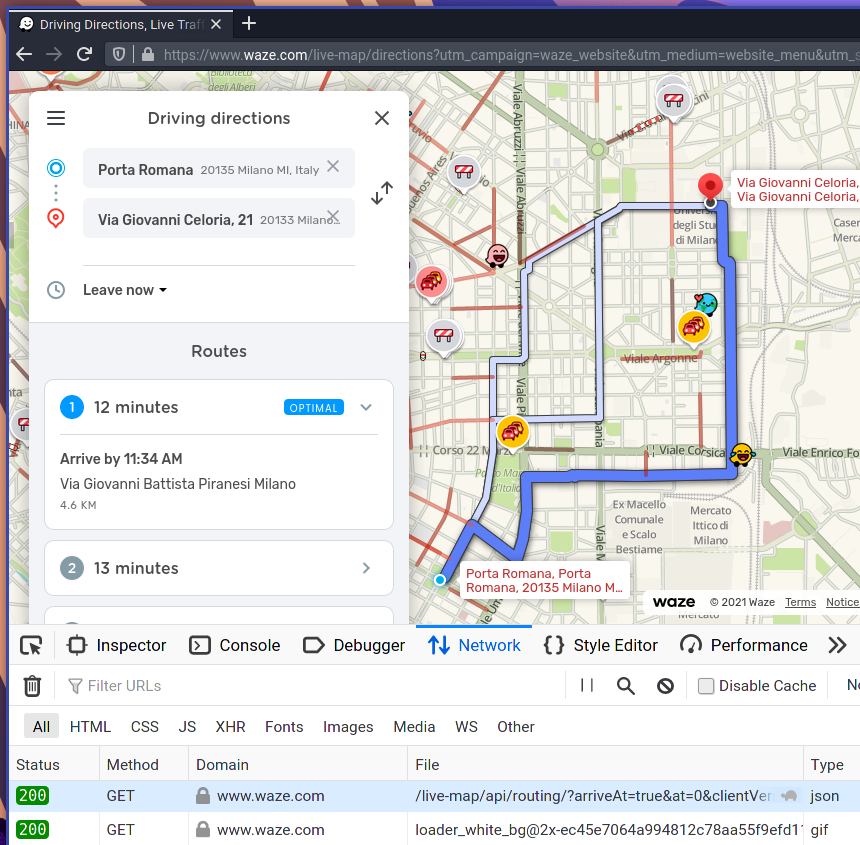
\includegraphics[scale=0.45]{waze_scraping}
\end{center}

in particolare, la richiesta verso l'url \url{https://www.waze.com/live-map/routing/?} contiene esattamente il punto di partenza e di arrivo richiesti parametrizzati nell'url della richiesta, e il risultato è restituito è in formato JSON. Per proteggere i loro server da sovraccarichi, Waze risponde a questo URL solamente se si possiede il permesso ricevuto preventivamente tramite un token, ovvero una stringa di caratteri che funge da chiave segreta. Per ottenere questa chiave e raggiungere l'obbiettivo finale di avere delle API per interrogare il servizio, è stato scritto un programma in Golang per emulare l'interazione col sito web e ricevere il token necessario per effettuare le richieste successive. Questo processo ha richiesto tempo sia per la codifica dei parametri e che per la decodifica del risultato stesso e dei risultati intermedi per la richiesta del token. In altre parole, è stato fatto il reverse engineering della web app.

\subsubsection{Stima del percorso per il car sharing}

Avendo trovato un modo per risolvere i tempi di percorrenza in auto, per il servizio di car sharing Enjoy si è scelto di calcolare una stima che tiene conto del raggiungimento a piedi dell'auto libera più vicino al luogo di partenza del viaggio e del tragitto in auto tra la posizione di quest'ultima e il luogo di destinazione. Nello specifico, ogni volta che viene richiesto un percorso, viene scaricata la lista aggiornata delle auto libere presenti sul territorio e viene scelta l'auto più vicina calcolando la distanza dal punto di partenza richiesto a ogni auto presente nella lista. Una voltra trovata la posizone dell'auto libera, vengono sommate la stima di percorrenza del raggiungimento di tale auto a piedi e la stima di percorrenza in auto dal luogo in cui si trova l'auto fino alla destinazione. Sebbene non sia l'approccio migliore, dato che non tiene conto della direzione e del verso di marcia per compiere il viaggio, e quindi rendendo possibile la scelta di auto più vicina al punto di partenza ma che si allontana dal luogo di destinazione, è risultato il più semplice da programmare e successivamente da testare.

\section{Scelta tra percorsi random e prefissati}

Si è scelto di usare diverse tratte su cui basare il confronto allo scopo di ricoprire a livello topografico una buona parte del Comune di Milano e di diversificare i confronti in base alle caratteristiche delle tratte, quali lunghezza, coordinate geografiche di partenza e destinazione, per simulare al meglio la posizione di un possibile utente nella mappa.

Per rendere automatiche le richieste da inoltrare ai servizi di navigazione è stata creata una sorgente dal quale pescare le tratte. Sono stati presi in considerazione tre principali approcci per creare tale sorgente: hard-coded random; hard-coded di tratte realmente percorse; generazione a random just-in-time. I primi due approcci sono risultati fin da subito problematici.

In primo luogo, la scelta della destinazione avrebbe introdotto bias cognitivi riguardo il possibile utente del percorso, portando ad analizzare la mobilità solamente dal punto di vista di una determinata categoria, per esempio: selezionando tratte con delle università come punto di arrivo porterebbe ad analizzare la mobilità solamente dal punto di vista degli studenti e dipendenti presso quelle determinate strutture. Altri problemi simili sarebbero sorti nello scegliere la partenza, la lunghezza, la distanza dal centro città e numerosità delle tratte.

Seconda problematica molto più rilevante è che, involontariamente, si sarebbero introdotti dei percorsi che avrebbero favorito un mezzo piuttosto che un altro. Nella città di Milano infatti si contanto numerosi tratti stradali di questo genere: strade con corsia preferenziale per mezzi pubblici e taxi; strade a singola corsia e con numerosi semafori (quindi più soggetta a incolonnamenti); tangenziali; tratte coperte da passanti ferroviari (più veloci delle metropolitane e con meno fermate). Tale scelta avrebbe portato ad analizzare dati non rappresentativi della città, con conseguenti risultati in un certo senso "falsati".

Usando l'approccio della generazione a random non solo si sarebbero evitati tali problemi, ma i problemi stessi si sarebbero trasformati in analisi da poter eseguire a posteriori, per esempio selezionando da tutte le tratte generate a random quelle che hanno portato nei pressi di un'università, o tratte che in linea d'aria hanno coperto particolari strade favorevoli a determinati mezzi di trasporto. Visti i vantaggi e la flessibilità dell'approccio, si è optato per quest'ultimo.

\section{Generatore random dei percorsi}

Prima ancora di scrivere una funzione per generare tratte a random è stata scelta l'area geografica all'interno della quale generarle. Siccome il servizio di car sharing Enjoy non permette di usare la propria flotta al di fuori del Comune di Milano, tale area è stata selezionata come terreno per i confronti, rappresentata sotto forma di rettangolo per questioni di semplicità nella programmazione. Nello specifico, sono state scelte le coordinate (45.450562\textdegree, 9.158959\textdegree) e (45.482032\textdegree, 9.206763\textdegree) rispettivamente come vertice in basso a sinistra e in alto a destra del rettangolo rappresentativo dell'area selezionata. In questo modo la generazione di punti a random è stata ridotta alla generazione di coordinate maggiori o uguali della prima e minori o uguali della seconda.

Una volta scritta la funzione per la generazione a random delle tratte, è stato introdotto un constraint per simulare dei percorsi scomodi da fare a piedi, ovvero per generare tratte che supererebbero i 20 minuti di camminata per essere coperte, e al tempo stesso che giustificherebbero l'utilizzo della macchina. Si è scelto di usare 2 km in linea d'aria dal punto di partenza a quello di destinazione come misura minima della lunghezza di una tratta.

Un secondo constraint è stato introdotto per avere una maggiore eterogeneità delle tratte generate a livello geografico. Molte delle linee principali dei mezzi pubblici infatti attraversano il centro storico di Milano, inoltre l'area del centro storico rappresenta più della metà dell'area selezionata dal constraint precedente. Siccome è stato scelto di ricoprire a livello topografico tutta l'area di Milano, si è programmato il generatore in modo da creare in maniera equidistribuita le seguenti tipologie di tratte: da dentro il centro storico a fuori; da dentro a dentro; da fuori a fuori; da fuori a dentro. Il rettangolo rappresentativo del centro storico è stato disegnato secondo i seguenti vertici: (45.450562\textdegree, 9.158959\textdegree), (45.482032\textdegree, 9.206763\textdegree).

\section{Timing delle richieste}

Le richieste sono state programmate per essere effettuate dalle 7:00 alle 23:59 di ogni giorno. La scelta di tale intervallo è stata vincolata dall'orario di servizio dei mezzi pubblici ATM, difatti in tale orario viene garantito il pieno regime del servizio, mentre vengono offerti collegamenti e passaggi saltuari al di fuori di esso.
Per rispettare i limiti giornalieri delle varie API si è scelto di effettuare 1 richiesta al minuto, dove ogni richiesta rappresenta un tragitto generato a random mandato simultaneamente a ogni servizio di navigazione per ottenere una stima da ognuno di essi, per un totale di circa 1,000 richieste al giorno. Oltre ai valori delle stime di percorrenza per ogni mezzo, insieme alla richiesta sono stati salvati altri dati come il numero di macchine libere enjoy al momento della richiesta, la distanza aerea della tratta e quella calcolata a piedi. 

\section{Pseudocodice del programma}

\begin{lstlisting}[language=Go]
var a, b, c coordinate

for {
	a, b = creaTragittoRandom()
	c = enjoy.trovaAutoPiuVicina(a)
	
	risultato := []stime{
		here.stimaTragitto(a, b),
		waze.stimaTragitto(a, b),
		osm.stimaTragitto(a, b, "foot"),
		osm.stimaTragitto(a, b, "bike"),
		osm.stimaTragitto(a, c, "foot") +
			waze.stimaTragitto(c, b)
	}
	
	save(risultato)
}
\end{lstlisting}